\section{Mission constraints}

% https://www.projectrho.com/public_html/rocket/infrastructure.php#eml1best

Despite simplifications, the mission design process is still a complex problem.
There exists a wide range of mission constraints that can be imposed on the
analysis to refine the results and make them more realistic. These include fuel
mass, characteristic energy, excess velocity at arrival, time of flight,
tracking constraints, and communication constraints. For a complete overview of
mission contraints, the reader is referred to \cite{smad2011}.

\subsection{Fuel mass}

The fuel mass is a critical constraint in mission design. For every impulse
performed by the spacecraft, a certain amount of fuel is consumed. This loss in
mass is modeled according to the Tsiolkovsky rocket equation \ref{eq:tsiolkovsky}:

\begin{equation}
  \Delta v = v_e \ln \left( \frac{m_0}{m_f} \right) = I_{sp} g_0 \ln \left( \frac{m_0}{m_f} \right)
  \label{eq:tsiolkovsky}
\end{equation}

Where $\Delta v$ is the change in velocity, $v_e$ is the exhaust velocity, $m_0$
is the initial mass of the spacecraft, $m_f$ is the final mass of the
spacecraft. Other variants of the expression include the $I_{sp}$, the specific
impulse of the propulsion system, and $g_0$, the standard gravity.

\subsection{Characteristic energy}

The characteristic energy $C_3$ is also a good estimator for the propulsion
requirements of a mission.

The $\Delta v$ relates with the characteristic energy $C_3$, also known as
specific energy. Equation \ref{eq:c3} summarizes this relation for hyperbolic
orbits:

\begin{equation}
  C_3 = v_{\infty}^2
  \label{eq:c3}
\end{equation}

Given a propulsion system, a maximum specific energy is imposed, limiting the
maximum $\Delta v$ that the spacecraft can achieve. If a spacraft can not reach
a certain characteristic energy, then the mission is not feasible and the
target orbit can not be achieved.

The specific energy at launch is related with the payload via
\ref{eq:tsiolkovsky}. Figure \ref{fig:payload_vs_c3} shows the maximum payload for a
given characteristic energy for various modern launchers.

\begin{figure}[H]
  \centering
  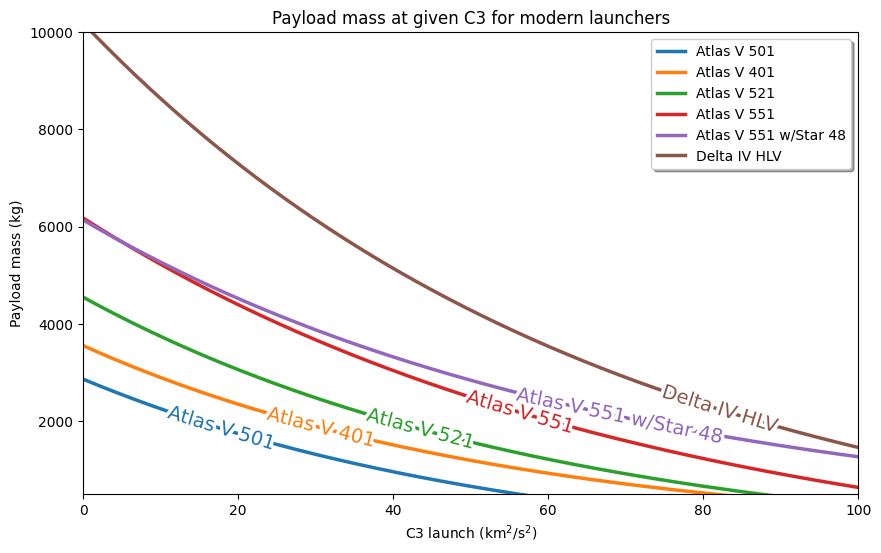
\includegraphics[width=\textwidth]{fig/static/payload_vs_c3}
   \caption[Maximum payload for a given characteristic energy for various modern]{Maximum payload for a given characteristic energy for various modern launchers.}
  \label{fig:payload_vs_c3}
\end{figure}

\subsection{Excess velocity at arrival}
\label{sec:excess_velocity}

Another mission constraint within the context of interlopers rendezvous is the
excess velocity at arrival. Lauch and arrival velocities are used to compute the
impulsed required to reach the target orbit. The first impulse $\Delta v_1$ is
used to launch the spacecraft into the target orbit. The second impulse $\Delta
  v_2$ is used to adapt to the orbit of the interloper, leading to a rendezvous.
Thus, two scenarios are possible:

\begin{itemize}

  \item \textbf{Targeting of the interloper.} The spacecraft overshoots the target by
        not applying the final impulse. This ahieves a greater launch
        impulse as more fuel mass can be allocated for this task. However, the
        spacecraft is not able to rendezvous with the interloper, as the second
        impulse is never applied.

  \item \textbf{Rendezvous with the interloper.} The spacecraft performs the
        arrival impulse to adapt to the orbit of the interloper. This reduces the
        amount of fuel available for the launch impulse but allows the spacecraft to
        follow the interloper.

\end{itemize}

Wether the spacecraft overshoots the target or rendezvous with the interloper,
the excess velocity at arrival is a critical parameter.

\subsection{Time of flight}

The time of flight is another important constraint in mission design. It refers
to the elapsed time between the launch and the rendezvous with the interloper.
Usually, short times of flight are preferred. They reduce the exposure to space
radiaiton, which can affect the spacecraft and its electronics. However, short
time of flights require greater fuel mass and thus greater propulsion to achieve
greater speeds for covering the astronomical distances between the launch and
arrival positions.

\subsection{Tracking constraints}

The spacecraft must be able to track the interloper and its own position
relative to the stars background. By doing so, the spacecraft can assert if it
is on the right orbit and if it is following the interloper correctly.

However, tracking a small object in deep space is a challenging task. For
example, 1I/'Oumuamua did not presented any cometary activity, having an absolute
magnitude of $M = 22$ (JPL SBDB) which made it difficult to observe and track
it. On the other hand, 2I/Borisov exhibited a coma, making it more visible by
having a magnitude of $M = 16$, see \cite{jewitt2020}.
